\documentclass[GBK,winfonts,a4paper,10pt]{ctexart}
\usepackage{fancyhdr}
\usepackage{indentfirst}
\usepackage{graphics}
\usepackage{enumerate}
\usepackage{framed}
\usepackage{amsmath}
\usepackage{graphicx}
\usepackage{setspace}
\usepackage{hyperref}
\usepackage{mdwlist}
\usepackage{algorithm}
\usepackage{algorithmic}
\usepackage{listings}
\usepackage{xcolor}
\usepackage{marvosym,listings,etoolbox}
\usepackage{geometry}

\lstset{numbers=left, numberstyle=\small, keywordstyle=\color{blue!70}, commentstyle=\color{red!50!green!50!blue!50}, frame=shadowbox, rulesepcolor=\color{red!20!green!20!blue!20},escapeinside=``, xleftmargin=2em,xrightmargin=2em, aboveskip=1em, literate={@}{\MVAt}1}

\patchcmd{\verb}{\dospecials}{\dospecials\atspecial}{}{}
\def\atspecial{\begingroup\lccode`~=`@
  \lowercase{\endgroup\let~}\MVAt
  \catcode`@=\active}
  


\newcommand{\tabincell}[2]{\begin{tabular}{@{}#1@{}}#2\end{tabular}}%
       
\lstdefinestyle{customc}{
  belowcaptionskip=1\baselineskip,
  breaklines=true,
  frame=single,
  xleftmargin=\parindent,
  language=C,
  showstringspaces=false,
  basicstyle=\fontsize{8pt}{8pt}\ttfamily,
  keywordstyle=\bfseries\color{green!40!black},
  commentstyle=\itshape\color{purple!40!black},
  identifierstyle=\color{blue},
  stringstyle=\color{orange},
  tabsize=4,
  numbers=none,
  mathescape=false,
}

\lstset{escapechar=@,style=customc}

\pagestyle{fancy}
\hypersetup{pdfborder=0 0 0}

\usepackage{clrscode}

\usepackage{latexsym}

\begin{document}

\rhead{}
\lhead{}
\cfoot{\thepage}
\renewcommand{\footrulewidth}{0.4pt}
%\renewcommand{\thesection}{}
\renewcommand{\algorithmicrequire}{\textbf{Input:}}
\renewcommand{\algorithmicensure}{\textbf{Output:}}
\setlength{\tabcolsep}{2pt}

\setlength{\parindent}{2em}

\thispagestyle{fancy}


\title{Operating System MIT 6.828 JOS Lab5 Report}
\author{Computer Science \\ ChenHao(1100012776) }
\date{\today}
\maketitle

\thispagestyle{fancy}

\tableofcontents

\newpage

\par
Lab5主要是要实现了一个简单的,只读,基于磁盘的文件系统,文件系统实际上是一个用户级的进程,其它用户进程对磁盘文件进行访问是通过和文件系统进程进行IPC通信来实现的。不过这个Lab材料太少了,看不太懂代码呀!
\par
Unix的文件系统将磁盘分为两个区域:inode和data区域。inode区域保存文件的状态属性,以及所指向数据块的指针,data区域存放文件的内容和元信息。
JOS磁盘由两个基本单位:扇区和块。磁盘中一般第一块或最后一块是Super Block,里面存放了包含文件系统的各项元数据,例如block的大小,磁盘大小,磁盘布局等。
\begin{section}{ Exercise 1 }
\par
x86处理器通过EFLAGS寄存器中的IOPL位来决定保护模式下是否可以执行特殊的I/O指令,因此我们需要给file system environment I/O权限,如果同时有多个environment享有I/O权限,则会对于中断的分配到对应的user-mode environment造成很大困扰。
\par
IOPL有4种特权级,其中0级的特权最高,3级最低,而此处是给予用户进程权限,因此给予FL\_IOPL\_3。
\begin{lstlisting}[language=C]
    if (type == ENV_TYPE_FS)
        e->env_tf.tf_eflags |= FL_IOPL_3;        
\end{lstlisting}
\end{section}

\begin{section}{ Question 1 }
\par
e->env\_tf会在产生trap时,由硬件以及中断处理程序进行保存,在env\_pop\_tf()中恢复。
\end{section}

\begin{section}{ Exercise 2 }
\par
Block Cache是物理磁盘上磁盘块的缓存,用来加速对磁盘的访问。JOS在文件系统进程中使用最多3G(DISKSIZE)内存在保存磁盘内容,从DISKMAP开始的3G来进行内存到磁盘空间的映射。开始并不会进行映射,只有在需要访问某个磁盘块的时候才会进行Block Cache。因此本质上这就是一个page fault handler,不同之处在于拷贝信息,一个是从内存中,这个是从硬盘中。
\par
在真实的文件系统中一般在会限制the block cache的大小,当超过大小的时候,则会将一部分磁盘块缓存写回磁盘块中。但是JOS的文件系统中并没有实现回收。
\begin{lstlisting}[language=C]
    	addr = ROUNDDOWN(addr, PGSIZE);
	r = sys_page_alloc(0, addr, PTE_W | PTE_U | PTE_P);
	if (r < 0) panic("bc_pgfault sys_page_alloc error : %e\n", r);

	r = ide_read(blockno * BLKSECTS, addr, BLKSECTS);
	if (r < 0) panic("bc_pgfault ide_read error : %e\n", r);       
\end{lstlisting}
\end{section}

\begin{section}{ Exercise 3 }
\par
这里JOS实现了一个简易的类似exec功能的过程——spaw。
spaw大致流程:从磁盘中打开文件,读取文件,调用sys\_exofork创建子进程,并设置子进程的trapframe以及初始化其栈空间,并将elf文件读入子进程相应内存位置,设置eip和esp,并设置为RUNNABLE即可。
\par
sys\_env\_set\_trapframe使得进程根据Trapframe来使某一个进程的状态变化,例如设置进程的eip和esp位置,从而实现类似exec的效果。
\begin{lstlisting}[language=C]      
static int
sys_env_set_trapframe(envid_t envid, struct Trapframe *tf)
{
	// LAB 5: Your code here.
	// Remember to check whether the user has supplied us with a good
	// address!
	struct Env * env;
	int r = envid2env(envid, &env, 1);
	if (r < 0) return -E_BAD_ENV;	

	user_mem_assert (env, tf, sizeof(struct Trapframe), PTE_U);

	env->env_tf = *tf;
	env->env_tf.tf_cs |= 3;
	env->env_tf.tf_eflags |= FL_IF;

	return 0;
}
\end{lstlisting}

\end{section}

\begin{section}{ \textcolor[rgb]{1.00,0.00,0.00}{Challenge 2: Unix-style exec} }
\par
\textcolor[rgb]{1.00,0.00,0.00}{这里提到了spawn会比Unix-style exec要容易实现,这是为什么呢?}
\par
注意到执行spawn的时候,实际上当前进程fork了一个子进程,然后将需要执行的elf文件导入至子进程。而Unix style exec是replaces the current process image with a new process image.是不通过fork的。这就是两者的区别,Unix-style exec是比较困难实现的,因为很可能需要执行的elf文件需要存放的虚拟内存位置会和当前进程的代码和数据冲突,而导致崩溃。
\par
那么真实的操作系统是如何做到的呢?通过动态链接,这样用户库的exec就不会被读入的静态数据和代码而覆盖掉。
\par
\par
赤手空拳难以写出动态链接,那么我们是不是可以实现一个伪动态链接,lab4中pgfault里面copy-on-write的时候通过临时页表进行保存。因此我们可以先把elf文件都存放在别的页面,等陷入kernel里面再移送到正确的位置。于是我很邪恶地将某一块地址 0x80000000开始的地方作为临时的缓冲区域。
\par
大致流程就是exec先将elf文件以及新的栈内容拷贝到临时内存中作为缓冲,再引发一个system call来实现将临时内存的内容拷贝至真是的地址上。因为在系统调用中处于内核,因此不用担心新的代码和数据将原用户代码和数据覆盖掉。
\par
在spawn.c中设置exec和execl函数,execl函数与spawnl几乎完全一样,exec如下。由于栈的内容不能马上进行覆盖,因此新的栈的内容也需要先放置在新的临时内存中。因此需要更改一下init\_stack函数中,即设置一下映射的地址即可。
\begin{lstlisting}[language = C]
// exec: Since I don't know how to built dynamic linking in JOS, so I use virtual address that starts from 
// 		 0x80000000(MYTEMPLATE) to be template block cache. Then sys_exec is a system call to complete 
// 		 memory setting.
// Remember: When there is virtual memory in ELF linking address overlaped with MYTEMPLATE, exec will fail.
int
exec(const char *prog, const char **argv)
{
	unsigned char elf_buf[512];
	uintptr_t tf_esp;

	int fd, i, r;
	struct Elf *elf;
	struct Proghdr *ph;
	int perm;	


	if ((r = open(prog, O_RDONLY)) < 0)
		return r;
	fd = r;

	// Read elf header
	elf = (struct Elf*) elf_buf;
	if (readn(fd, elf_buf, sizeof(elf_buf)) != sizeof(elf_buf)
	    || elf->e_magic != ELF_MAGIC) {
		close(fd);
		cprintf("elf magic %08x want %08x\n", elf->e_magic, ELF_MAGIC);
		return -E_NOT_EXEC;
	}


	// Set up program segments as defined in ELF header.
	uint32_t now_addr = MYTEMPLATE;
	ph = (struct Proghdr*) (elf_buf + elf->e_phoff);
	for (i = 0; i < elf->e_phnum; i++, ph++) {
		if (ph->p_type != ELF_PROG_LOAD)
			continue;
		perm = PTE_P | PTE_U;
		if (ph->p_flags & ELF_PROG_FLAG_WRITE)
			perm |= PTE_W;
		if ((r = map_segment(0, PGOFF(ph->p_va) + now_addr, ph->p_memsz,
				     fd, ph->p_filesz, ph->p_offset, perm)) < 0)
			goto error;
		now_addr += ROUNDUP(ph->p_memsz + PGOFF(ph->p_va), PGSIZE);
	}
	close(fd);
	fd = -1;

	// Set up Stack 
	if ((r = init_stack(0, argv, &tf_esp, now_addr)) < 0)
		return r;

	// Syscall
	if (sys_exec(elf->e_entry, tf_esp, (void *)(elf_buf + elf->e_phoff), elf->e_phnum) < 0)
		goto error;
	return 0;
	
error:
	sys_env_destroy(0);
	close(fd);
	return r;
}
\end{lstlisting}

\par
设置新的system call,sys\_exec。将临时内存中的内容移动到真实的地址中,以及构建新的栈内容。代码如下:
\begin{lstlisting}[language = C]
static int
sys_exec(uint32_t eip, uint32_t esp, void * v_ph, uint32_t phnum)
{
	// set new eip and esp
	memset((void *)(&curenv->env_tf.tf_regs), 0, sizeof(struct PushRegs));
	curenv->env_tf.tf_eip = eip;
	curenv->env_tf.tf_esp = esp;

	int perm, i;
	uint32_t now_addr = MYTEMPLATE;
	uint32_t va, end_addr;
	struct PageInfo * pg;

	// Elf 
	struct Proghdr * ph = (struct Proghdr *) v_ph; 
	for (i = 0; i < phnum; i++, ph++) {
		if (ph->p_type != ELF_PROG_LOAD)
			continue;
		perm = PTE_P | PTE_U;
		if (ph->p_flags & ELF_PROG_FLAG_WRITE)
			perm |= PTE_W;

		// Move to real virtual address
		end_addr = ROUNDUP(ph->p_va + ph->p_memsz, PGSIZE);
		for (va = ROUNDDOWN(ph->p_va, PGSIZE); va != end_addr; now_addr += PGSIZE, va += PGSIZE) {
			if ((pg = page_lookup(curenv->env_pgdir, (void *)now_addr, NULL)) == NULL) 
				return -E_NO_MEM;		// no page
			if (page_insert(curenv->env_pgdir, pg, (void *)va, perm) < 0)
				return -E_NO_MEM;		
			page_remove(curenv->env_pgdir, (void *)now_addr);
		}
	}

	// New Stack
	if ((pg = page_lookup(curenv->env_pgdir, (void *)now_addr, NULL)) == NULL) 
		return -E_NO_MEM;
	if (page_insert(curenv->env_pgdir, pg, (void *)(USTACKTOP - PGSIZE), PTE_P|PTE_U|PTE_W) < 0) 
		return -E_NO_MEM;
	page_remove(curenv->env_pgdir, (void *)now_addr);
	
	env_run(curenv);		// never return
	return 0;
}
\end{lstlisting}

\par
测试:利用spawnhello.c来测试,对于原始的spawnhello,在最后增加一行I come back!。
\begin{lstlisting}[language = C]
#include <inc/lib.h>

void
umain(int argc, char **argv)
{
	int r;
	cprintf("i am parent environment %08x\n", thisenv->env_id);
	if ((r = spawnl("hello", "hello", 0)) < 0)
		panic("spawn(hello) failed: %e", r);
	cprintf("I come back!\n");
}
\end{lstlisting}
\par
则结果应该是会执行"hello.c"并且会输出I come back!,因为spawn是基于fork的。结果符合预期
\par
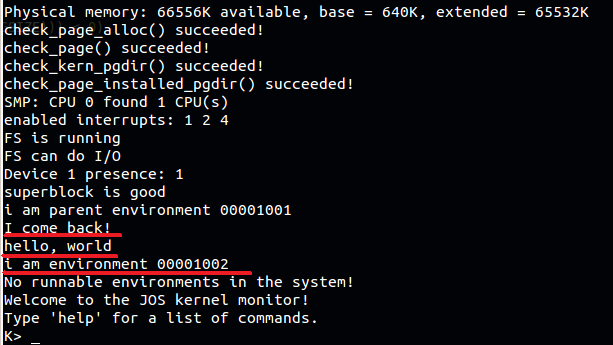
\includegraphics[scale=0.5]{ch1.png}
\par
将spawnhello改为exec,即:
\begin{lstlisting}[language = C]
#include <inc/lib.h>

void
umain(int argc, char **argv)
{
	int r;
	cprintf("i am parent environment %08x\n", thisenv->env_id);
	if ((r = execl("hello", "hello", 0)) < 0)
		panic("spawn(hello) exec: %e", r);
	cprintf("I come back!\n");
}
\end{lstlisting}
\par
则结果应该会执行"hello.c"并且不会有输出I come back,以及exec的进程号与原进程号一样。结果符合预期
\par
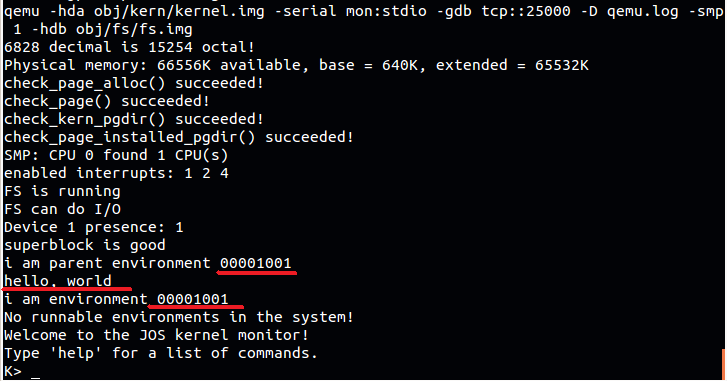
\includegraphics[scale=0.5]{ch2.png}
\end{section}

\begin{section}{ Exercise 4 }
\par
还记得在以前的fork中,采用了Copy-on-write的技术,因此需要在将PTE\_W或者PTE\_COW的页面标记为PTE\_COW。而对于文件,由于file descriptor是共享的,因此在duppage考虑一下PTE\_SHARE即可。
\begin{lstlisting}[language = C]
static int
duppage(envid_t envid, unsigned pn)
{
	// do not dup exception stack
	if (pn * PGSIZE == UXSTACKTOP - PGSIZE) return 0;

	int r;
	void * addr = (void *)(pn * PGSIZE);
    if (uvpt[pn] & PTE_SHARE) {
        r = sys_page_map(0, addr, envid, addr, uvpt[pn] & PTE_SYSCALL);
        if (r < 0) panic("duppage sys_page_map error : %e\n", r);
    } else
	if ((uvpt[pn] & PTE_W) || (uvpt[pn] & PTE_COW)) {
		// cow
		r = sys_page_map(0, addr, envid, addr, PTE_COW | PTE_P | PTE_U);
		if (r < 0) panic("duppage sys_page_map error : %e\n", r);
		
		r = sys_page_map(0, addr, 0, addr, PTE_COW | PTE_P | PTE_U);
		if (r < 0) panic("duppage sys_page_map error : %e\n", r);
	} else {
		// read only
		r = sys_page_map(0, addr, envid, addr, PTE_P | PTE_U);
		if (r < 0) panic("duppage sys_page_map error : %e\n", r);
	}

	return 0;
}
\end{lstlisting}
\par
类似上一部分,对于spawn也需要进行这部分的映射。
\begin{lstlisting}[language = C]
// Copy the mappings for shared pages into the child address space.
static int
copy_shared_pages(envid_t child)
{
	// LAB 5: Your code here.
    uint32_t i;
    int r;
    for (i = 0; i != UTOP; i += PGSIZE) 
    if ((uvpd[PDX(i)] & PTE_P) && (uvpt[i / PGSIZE] & PTE_P) && (uvpt[i / PGSIZE] & PTE_SHARE)) {
        r = sys_page_map(0, (void *)i, child, (void *)i, uvpt[i / PGSIZE] & PTE_SYSCALL);
        if (r < 0) return r;
    }
	return 0;
}
\end{lstlisting}
\end{section}

\begin{section}{ Exercise 5 }
\par
这部分比较简单,增加trap处理判断即可。
\end{section}

\begin{section}{ Question 2 }
\par
2. About 10 hours.
\par
3. 这部分的exercise比较少,需要看的代码比较多,对于file I/O有了解,但是因为经过写的训练,总觉的有点陌生。
\end{section}

\par
make grade纪念,所有lab做完了:
\par
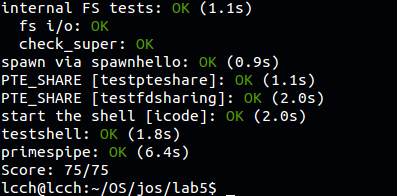
\includegraphics[scale=0.5]{lab5makegrade.png}
\begin{section}{ Summary }
\par
这个Lab是JOS中的最后一个Lab,Exercise比较少,最后实现起来的代码也少,基本上按照注释就可以实现了。而这个Lab提到的JOS中的文件系统,因为在做这个Lab的时候,对于文件系统还不是很熟悉,而且这个Lab并没有很多预备的材料,因此花了许多时间在查找资料上面。在大致了解了Unix的文件系统的原理和结构之后,又花了非常多的时间在看JOS实现的文件系统上面,这一部分Lab中并没有很多地提到,而且代码量比较大,因此对于阅读代码对我造成了一定的困难,在这个Lab中我花在查资料以及阅读代码的时间远远多于写Exercise的时间。并且到现在我对文件系统中的代码也没有完全吃透,还是有一些只能明白个大概。
\par
在完成了Lab5后,基本上就结束了本学期的操作系统实习,在不断地做Lab的过程中,对如何实现一个操作系统有了即宏观又细节的了解。很大地锻炼了我的代码阅读能力以及代码编写和调试bug的能力。通过代码阅读,我感觉到很多底层代码有一定的trick,以及一些很巧妙的实现的地方,以及对c语言和汇编有了更深的理解,对我以后代码能力有了很大的提高。在系统编程中,遇到bug非常麻烦而且非常耗时,由于系统编程所涉及到的代码量和文件量比较大,而且许多bug的重现率很低,因此遇到bug真是一个非常头疼的事情。通过5个Lab的锻炼,我总结出遇到bug,首先要自己对这个系统要比较清楚,这样对于bug才可能有一定的判断,另外在调试bug中我大量使用输出调试,通过输出调试来看每一阶段的状态,我感觉这个调试方法在我做Lab中帮助非常大。
\par
最后,终于把Lab都做完了,哈哈哈,非常开心。
\end{section}



\end{document}



















